\documentclass[12pt]{article}
\usepackage[english]{babel}
\usepackage[utf8x]{inputenc}
\usepackage{amsmath}
\DeclareMathOperator{\sign}{sign}
\usepackage{bm}
\usepackage{graphicx}
% \usepackage{biblatex}
% \bibliographystyle{ieeetr}
\usepackage[colorinlistoftodos]{todonotes}
\usepackage{float}
\usepackage[margin=0.75in]{geometry}
\usepackage{multirow}
%% Set double spacing
\usepackage{setspace}
\doublespacing

\setcounter{MaxMatrixCols}{20}

\usepackage{matlab-prettifier}
\onehalfspacing
\usepackage{lscape}
\usepackage{caption}
\usepackage{indentfirst}
% \usepackage{subfigure}
\usepackage{subcaption}
%\usepackage{times}
% \usepackage{fontspec}
\usepackage{indentfirst}
\usepackage{hyperref}
\usepackage{xcolor}
\hypersetup{
    colorlinks,
    linkcolor={red!1!black},
    citecolor={blue!1!black},
    urlcolor={blue!1!black}
}
%\setmainfont{times}
\renewcommand{\familydefault}{\rmdefault}

\title{MAE6780_Final_Report}

\begin{document}

\begin{titlepage}

\newcommand{\HRule}{\rule{\linewidth}{0.5mm}} % Defines a new command for the horizontal lines, change thickness here

\center % Center everything on the page
 
%----------------------------------------------------------------------------------------
%	HEADING SECTIONS
%----------------------------------------------------------------------------------------


\textsc{\Large MAE 6780}\\[0.5cm] % Major heading such as course name
\textsc{\large Cornell University}\\[0.5cm] % Minor heading such as course title

%----------------------------------------------------------------------------------------
%	TITLE SECTION
%----------------------------------------------------------------------------------------

\HRule \\[0.4cm]
{ \huge \bfseries Stabilization of a Quadrotor Drone from Random Initial Conditions Using Integral Sliding Mode Control}\\[0.4cm] % Title of your document
\HRule \\[1.5cm]
 
%----------------------------------------------------------------------------------------
%	AUTHOR SECTION
%----------------------------------------------------------------------------------------

\begin{minipage}{0.4\textwidth}
\begin{flushleft} \large
\emph{Author:}\\
Mitchell \textsc{Dominguez}\\
\emph{Group Members:}\\
Amlan \textsc{Sinha}\\
Patrick \textsc{Voorhees}\\
\end{flushleft}
\end{minipage}
~
\begin{minipage}{0.4\textwidth}
\begin{flushright} \large
\emph{NetID:} \\
md697\\
\vspace{23pt}
as2558\\
pwv9\\
\end{flushright}
\end{minipage}\\[2cm]
~
\begin{minipage}{0.4\textwidth}
\begin{center} \large
\emph{Instructor:}\\
Silvia Ferrari\\
\end{center}
\end{minipage}
%\linebreak
\linebreak
\linebreak

% If you don't want a supervisor, uncomment the two lines below and remove the section above
%\Large \emph{Author:}\\
%John \textsc{Smith}\\[3cm] % Your name

%----------------------------------------------------------------------------------------
%	DATE SECTION
%----------------------------------------------------------------------------------------

{\large 11 May, 2018}\\[2cm]


%----------------------------------------------------------------------------------------

\vfill % Fill the rest of the page with white space

\end{titlepage}
\newpage

\newpage
\tableofcontents{}
\newpage

\begin{abstract}
\normalsize
Quadrotor drones are incredibly versatile machines that have uses in everything from recreation to military applications. As such, the control of such vehicles is an incredibly relevant and important problem to solve. In this paper, integral sliding mode control is implemented to stabilize a quadrotor drone. Since the quadrotor is underactuated, with six degrees of freedom but only four actuators, the attitude and height of the drone can be directly controlled while the horizontal position is brought to a constant. The stability of the controller is proved through Lyapunov stability theory, and the controller is shown through simulation to achieve stability of the controlled states of the quadrotor, even under extreme initial conditions such as the drone being thrown into the air upside down. However, the presence of steady state errors in the controlled states results in unwanted motion in the horizontal plane, which will require further tuning of the controller and development of position control to eliminate.
\end{abstract}

\newpage
\section{Introduction and Theory}
\subsection{Overview}
Since the normal operation of a quadcopter does not involve much deviation in the roll, pitch, and yaw angles from those in the hovering condition, it is often convenient to design controllers for quadcopters based on linearizations of the equations of motion about the hovering condition. However, the goal of stabilizing the quadcopter under any set of initial conditions necessarily means that the quadcopter will experience states far from the hovering condition. Thus designing a linear controller to achieve the robust stabilization of the quadcopter would involve linearizing about several states and implementing a form of gain scheduling, which would be quite complex and impractical.

In this paper, an integral sliding mode controller is developed to control the quadcopter using the full nonlinear equations of motion of the vehicle. This approach avoids the problems that arise from dealing with linearized systems, namely that any linearization of a nonlinear system is only useful within certain bounds. Outside these bounds, the linearized model would cease to be accurate and any control law applied in the situation would be useless. A nonlinear control law such as sliding mode control does not suffer from these same issues, and thus is ideal for applications such as this.

\subsection{Nonlinear Dynamics of the Quadrotor}
The position and attitude of a quadcopter in inertial space is described by $[\begin{matrix} x & y & z & \phi & \theta & \psi\end{matrix}]^T$, where x,y, and z correspond to the Cartesian position of the vehicle, and $\phi$, $\theta$, and $\psi$ are the roll, pitch, and yaw angles that correspond to a 1-2-3 Euler angle set.

The dynamics of the quadrotor were initially derived relative to the body-frame rates $[\begin{matrix} u & v & w & p & q & r\end{matrix}]^T$ corresponding to velocities in the body x,y, and z directions and angular velocities about the body x,y, and z directions respectively. These equations can be seen in Equation \ref{eq:bodyEOM}, where $I_x$, $I_y$, and $I_z$ correspond to the moments of inertia of the quadcopter about its body axes, $J_R$ is the rotor moment of inertia, $g$ is the acceleration due to gravity, $L$ is the length of each arm of the quadcopter, $\Omega = -\Omega_1 + \Omega_2 - \Omega_3 + \Omega_4$ is a combination of the rotor speeds $\Omega_i$, and $U_i$ correspond to the control inputs which are defined in the next section.

\begin{centering}
\begin{align} \label{eq:bodyEOM}
\begin{split}
\dot{u} &= (vr-wq) + g\sin\theta\\
\dot{v} &= (wp-ur)-g\sin\phi\cos\theta\\
\dot{w} &= (uq - vp) - g\cos\phi\cos\theta + \frac{U1}{m}\\
\dot{p} &= \left(\frac{I_y - I_z}{I_x}\right)qr - \frac{J_R}{I_x}q\Omega + \frac{L}{I_x}U_2\\
\dot{q} &= \left(\frac{I_z-I_x}{I_y}\right)pr + \frac{J_R}{I_y}p\Omega + \frac{L}{I_y}U_3\\
\dot{r} &= \left( \frac{I_x - I_y}{I_z} \right)pq + \frac{1}{I_z}U_4
\end{split}
\end{align}
\end{centering}

While the body-frame equations are sufficient to bring all of the quadrotor's positional and angular rates to zero, they are however insufficient to stabilize the inertial positions and angles. Thus, a conversion to inertial equations of motion is necessary. This was done by making the assumption that the angular rates are small, resulting in $p \approx \dot{\phi}$, $q \approx \dot{\theta}$, and $r \approx \dot{\psi}$. Applying this assumption, the inertial equations of motion in (\ref{eq:inertialEOM}) were thus derived \cite{SudhirSwarup}.

\begin{centering}
\begin{align} \label{eq:inertialEOM}
\begin{split}
\ddot{x} &= \frac{U_1}{m}\left(\cos\phi\sin\theta\cos\psi + \sin\phi\sin\psi\right)\\
\ddot{y} &= \frac{U_1}{m}\left(\cos\phi\sin\theta\sin\psi - \sin\phi\cos\psi\right) \\
\ddot{z} &= \frac{U_1}{m}\left(\cos\phi\cos\psi\right) -g\\
\ddot{\phi} &= \left(\frac{I_y - I_z}{I_x}\right)\dot{\theta}\dot{\psi} - \frac{J_R}{I_x}\dot{\theta}\Omega + \frac{L}{I_x}U_2\\
\ddot{\theta} &= \left(\frac{I_z-I_x}{I_y}\right)\dot{\phi}\dot{\psi} + \frac{J_R}{I_y}\dot{\phi}\Omega + \frac{L}{I_y}U_3\\
\ddot{\psi} &= \left( \frac{I_x - I_y}{I_z} \right)\dot{\theta}\dot{\phi} + \frac{1}{I_z}U_4
\end{split}
\end{align}
\end{centering}

The system was then integrated by using the following state:

\begin{centering}
\begin{equation}
\bm x = \begin{bmatrix}
x & \dot{x} & y & \dot{y} & z & \dot{z} & \phi & \dot{\phi} & \theta & \dot{\theta} & \psi & \dot{\psi}
\end{bmatrix}^T
\end{equation}
\end{centering}


\subsection{Definition of Control Inputs}
In the physical implementation of a quadcopter, voltage is provided to the motors to change the rotor speeds. The relation between voltage and rotor speed is shown in Equation \ref{eq:V2W}.

\begin{centering}
\begin{equation} \label{eq:V2W}
\bm{\Omega} =
\begin{bmatrix}
\Omega_1 \\ \Omega_2 \\ \Omega_3 \\ \Omega_4
\end{bmatrix}
=
\begin{bmatrix}
a_1 & 0 & 0 & 0\\
0 & a_2 & 0 & 0\\
0 & 0 & a_3 & 0\\
0 & 0 & 0 & a_4
\end{bmatrix}
\begin{bmatrix}
V_1 \\ V_2 \\ V_3 \\ V_4
\end{bmatrix}
+
\begin{bmatrix}
b_1 \\ b_2 \\ b_3 \\ b_4
\end{bmatrix}
=
A_V\bm{V} + \bm{b}
\end{equation}
\end{centering}

To relate the control inputs to rotor speed, however, a different relation is necessary. Equation \ref{eq:U2W} relates the control inputs $U_i$ to the rotor speeds, where $b$ is the coefficient of thrust and $d$ is the coefficient of drag \cite{twisty}. $U_1$ corresponds to thrust, and $U_2$, $U_3$, and $U_4$ correspond to the roll, pitch, and yaw moments respectively. 

\begin{centering}
\begin{equation} \label{eq:U2W}
\bm{U} = 
\begin{bmatrix}
U_1 \\ U_2 \\ U_3 \\ U_4
\end{bmatrix}
=
\begin{bmatrix}
b(\Omega_1^2 + \Omega_2^2 + \Omega_3^2 + \Omega_4^2)\\
b(\Omega_4^2-\Omega_2^2)\\
b(\Omega_3^2 - \Omega_1^2)\\
d(\Omega_4^2 + \Omega_2^2 - \Omega_3^2 - \Omega_1^2)
\end{bmatrix}
=
\begin{bmatrix}
b & b & b & b\\
0 & -b & 0 & b\\
-b & 0 & b & 0\\
-d & d & -d & d
\end{bmatrix}
\begin{bmatrix}
\Omega_1^2 \\ 
\Omega_2^2 \\
\Omega_3^2 \\
\Omega_4^2
\end{bmatrix}
=
A_U\bm{\Omega^2}
\end{equation}
\end{centering}

One of the major constraints on the system is that the actuators are not always able to provide the rotation rates that are called for by the controllers. This is because the quadrotor is a physical system where there are physical limits on the voltage that can be supplied to the motors and the speed with which the rotors can spin. Thus, as will be described later in the procedure section, the Simulink model for the controlled quadrotor has saturation blocks to simulate the physical saturation of the actuators on an actual drone.

Additionally, it is evident that there are only four control inputs, whereas the equations of motion dictate that there are six degrees of freedom in this system. Thus, this is an underactuated system. Four out of the six degrees of freedom can be chosen to be controlled, and the other two can only be stabilized. Since the goal of this project was to stabilize the attitude and height of the quadrotor, the roll, pitch, yaw, and height of the quadrotor were chosen as the controlled states. The result of this choice of controlled variables was of course that there was no explicit control of the position of the quadrotor in the horizontal plane. 


\section{Procedure}
\subsection{Derivation of the Control Law}
A system under sliding mode control evolves in two phases: the reaching mode and the sliding mode. This is illustrated in Figure \ref{fig:SMC_visualization}. The reaching mode involves forcing the system onto a sliding surface which is defined such that the system is asymptotically stable when on the surface. Once the system arrives on the sliding surface, it then needs to stay there for all time. This is the sliding mode \cite{SMCControlObservation}.

Following from these characteristics of sliding mode control, it follows that there are two main phases to designing a sliding mode controller. The first involves finding a manifold of asymptotic stability in the error space of the system. Such a manifold ensures that the error goes to zero. Once the sliding surface is defined, a control law that both drives the system to the sliding surface and then keeps it there must be designed\cite{SMCControlObservation}.

\begin{center}
\begin{figure}[H]
\captionsetup{width=.8\textwidth}
\centering
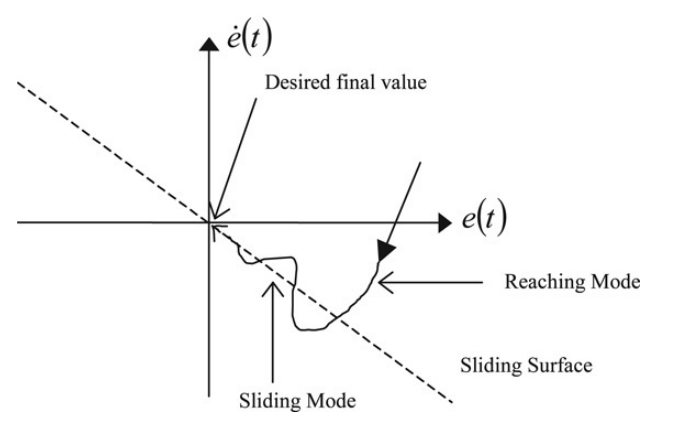
\includegraphics[width=0.70\textwidth]{SMC_visualization.PNG}
\caption{\label{fig:SMC_visualization}Visualization of sliding mode control \cite{camacho}.}
% From "Some long time delay sliding mode control approaches" by Oscar Camacho∗
% , Ruben Rojas ´ , Winston Garc´ıa-Gab´ın
\end{figure}
\end{center}

For integral sliding mode control, the sliding surface and its derivative can be defined as \cite{SMCControlObservation}:

\begin{center}
\begin{equation} \label{eq:s_definition}
\begin{split}
\sigma(\bm x(t)) &= k_p\bm e(t) + k_d\dot{\bm e}(t) + k_i\int_{t_0}^t\bm e(\tau)d\tau\\
\dot{\sigma}(\bm x(t)) &= k_p\dot{\bm e}(t) + k_d\ddot{\bm e}(t) + k_i\bm e(t)
\end{split}
\end{equation}
\end{center}

Lyapunov stability theory is then used to prove the asymptotic stability of the sliding surface and to derive the corresponding control law. A function $V(\bm x(t))$ is a Lyapunov function if it satisfies the following criteria:

\begin{centering}
\begin{equation} \label{eq:lyapunov}
\begin{split}
V(\bm x(t)) &= 0 \ \ \forall \ \ \bm x(t) = 0 \\
V(\bm x(t)) &> 0 \ \ \forall \ \ \bm x(t) \neq 0 \\
\dot{V}(\bm x(t)) &\leq 0 \ \ \forall \ \ \bm x(t) \neq 0
\end{split}
\end{equation}
\end{centering}

A candidate Lyapunov function must be equal to zero when $\bm x(t) = 0$ and must be positive definite for all nonzero values of $\bm x(t)$. Additionally, the time derivative of the Lyapunov function must be negative semidefinite for all nonzero states. If there exists a Lyapunov function for the system, then it can be said that the system is asymptotically stable \cite{khalil}. As the sliding surface must be asymptotically stable, a Lyapunov function for the system must be found.

A quadratic candidate Lyapunov function is often a good choice to ensure asymptotic stability \cite{SudhirSwarup}. As such, the candidate Lyapunov function is defined below:

\begin{center}
\begin{equation}
\begin{split}
V(\bm x(t)) &= \frac{1}{2}\sigma^T\sigma\\
\dot{V}(\bm x(t)) &= \sigma\dot{\sigma}
\end{split}
\end{equation}
\end{center}

The Lyapunov function candidate is positive semidefinite, so the first two Lyapunov stability criteria are achieved. Now the time derivative of the candidate Lyapunov function must be constrained to be negative semidefinite. It can be shown \cite{SMCControlObservation} \cite{SudhirSwarup} that if we set

\begin{center}
\begin{equation} \label{eq:sig_func}
\dot{\sigma}(\bm x(t)) = -k\sign(\sigma) - \eta\sigma
\end{equation}
\end{center}

then $\dot{V}(\bm x(t)) = -\kappa\sigma\sign(\sigma) - \eta\sigma^2 \leq 0$. Thus, setting the time derivative of the sliding surface equal to the expression in Equation \ref{eq:sig_func} yields a Lyapunov function for the sliding surface. Thus, applying Equation \ref{eq:sig_func} to the definition of the sliding surface yields an asymptotically stable system in the error space of the system.

The presence of the $\sign$ function in Equation \ref{eq:sig_func} makes this the "switching function" of the sliding mode controller. The function changes sign depending on the sign of the sliding variable $\sigma$ to always drive the system in the direction of the sliding manifold when it is not already on it. However, the use of the $\sign$ function tends to introduce a phenomenon called chattering in the sliding mode controller \cite{SMCControlObservation}. This is demonstrated in Figure \ref{fig:SMC_visualization} by the oscillation of the system state around the sliding surface. 

Chattering is an undesirable phenomenon because of the large control effort at all times necessary to combat it. Thus, in the implementation of sliding mode control, smoother alternatives to the $\sign$ function are often used \cite{SMCControlObservation}. In this project, the hyperbolic tangent function was selected as the alternative to the $\sign$ function to reduce the chattering phenomenon.

Applying the substitution in Equation \ref{eq:sig_func} and replacing $\sign$ with $\tanh$ yields
\begin{center}
\begin{equation}
k_p\dot{e}(t) + k_d\ddot{e}(t) + k_ie(t) = -\kappa\tanh(\sigma) - \eta\sigma
\end{equation}
\end{center}

Substituting in the error in the state $\bm e(t) = \bm x_d(t) - \bm x(t)$ yields

\begin{equation}
k_p\left(\dot{\bm x}_d(t) - \dot{\bm x}(t)\right) + k_d\left(\ddot{x}_d(t) - \ddot{x}(t) + k_i\left(\bm x_d(t) - \bm x(t)\right)\right) = -\kappa\tanh(\sigma) - \eta\sigma
\end{equation}

Substituting the equations of motion $\ddot{\bm x}$ from Equation \ref{eq:inertialEOM}, the control inputs can be derived to be the following:

\begin{align} \label{eq:U}
\begin{split}
U_1 &= \frac{m}{\cos\phi\cos\theta}\left(g+\ddot{z}_d+\frac{k_{p_z}}{k_{d_z}}(\dot{z}_d-\dot{z})+\frac{k_{i_z}}{k_{d_z}}(z_d-z)+\frac{\kappa_z}{k_{d_z}}\tanh(\sigma_z)+\frac{\eta_z}{k_{d_z}}\sigma_z\right) \\
U_2 &= \frac{I_{xx}}{L}\left(-\frac{I_{yy}-I_{zz}}{I_{xx}}\dot{\theta}\dot{\psi}+\frac{J_R}{I_{xx}}\dot{\theta}\Omega + \ddot{\phi}_D+\frac{k_{p_\phi}}{k_{d_\phi}}(\dot{\phi}_d-\dot{\phi})+\frac{k_{i_\phi}}{k_{d_\phi}}(\phi_d-\phi)+\frac{\kappa_\phi}{k_{d_\phi}}\tanh(\sigma_\phi)+\frac{\eta_\phi}{k_{d_\phi}}\sigma_\phi\right) \\
U_3 &= \frac{I_{xx}}{L}\left(-\frac{I_{zz}-I_{xx}}{I_{yy}}\dot{\phi}\dot{\psi}+\frac{J_R}{I_{xx}}\dot{\phi}\Omega + \ddot{\theta}_D+\frac{k_{p_\theta}}{k_{d_\theta}}(\dot{\theta}_d-\dot{\theta})+\frac{k_{i_\theta}}{k_{d_\theta}}(\theta_d-\phi)+\frac{\kappa_\theta}{k_{d_\theta}}\tanh(\sigma_\theta)+\frac{\eta_\theta}{k_{d_\theta}}\sigma_\theta\right) \\
U_4 &= I_{zz}\left(\frac{I_{xx}-I_{yy}}{I_{zz}}\dot{\phi}\dot{\theta}+\ddot{\psi}_D+\frac{k_{p_\psi}}{k_{d_\psi}}(\dot{\psi}_d-\dot{\psi})+\frac{k_{i_\psi}}{k_{d_\psi}}(\psi_d-\psi)+\frac{\kappa_\psi}{k_{d_\psi}}\tanh(\sigma_\psi)+\frac{\eta_\psi}{k_{d_\psi}}\sigma_\psi\right)
\end{split}
\end{align}

All $k$, $\kappa$, and $\eta$ values are tunable parameters that are used to optimize the performance of the controller through repeated simulations. Thus, there are 20 tunable parameters that can be adjusted to optimize the controller.

\subsection{Simulation of the Quadrotor System}
\subsubsection{Top-Level Block Diagram}
The controlled quadrotor system was simulated using Mathworks Simulink software. The top-level block diagram of the controller can be shown in the below figure:

\begin{center}
\begin{figure}[H]
\captionsetup{width=1\textwidth}
\centering
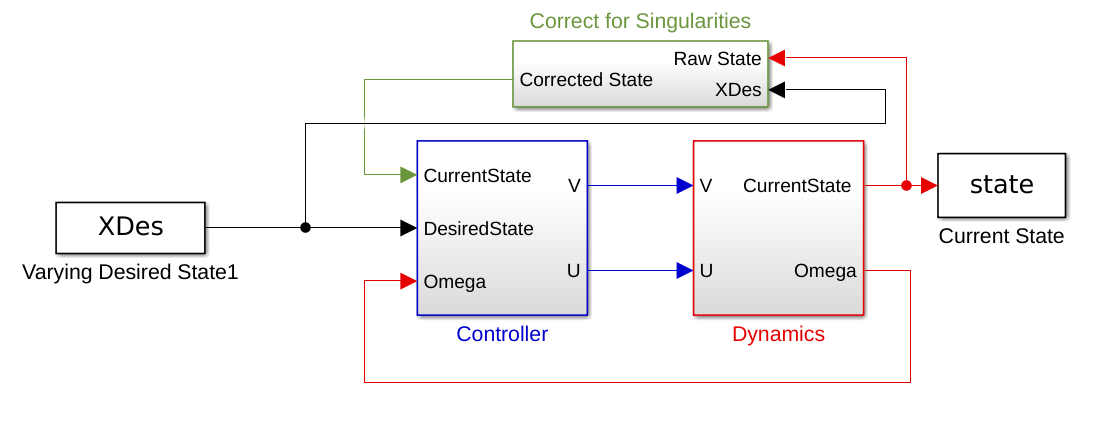
\includegraphics[width=0.70\textwidth]{overview.png}
\caption{\label{fig:overview}Top-level block diagram}
\end{figure}
\end{center}

The desired state, corrected current state, and the current $\Omega$ are all fed into the controller block, which then calculates corresponding voltages and control inputs. Those are then fed into the dynamics block, which outputs the updated state and $\Omega$ value. The current state goes through the correction block to account for singularities at $\phi = \frac{\pi}{2}$ and $\theta = \frac{\pi}{2}$. This is discussed in greater detail in Section \ref{sec:singularity_rejection}.

\subsubsection{Controller Block Diagram}
The block diagram of the controller is shown below in Figure \ref{fig:controller}. As can be seen from the figure, the corrected state, desired state, and $\Omega$ value is fed into the \texttt{sliding surface generator} block, which generates the sliding surfaces as defined in Equation \ref{eq:s_definition}. Then, the desired state, corrected current state, their derivatives, the sliding surface values, and $\Omega$ are fed into the \texttt{calculateU} block. 

\begin{center}
\begin{figure}[H]
\captionsetup{width=1\textwidth}
\centering
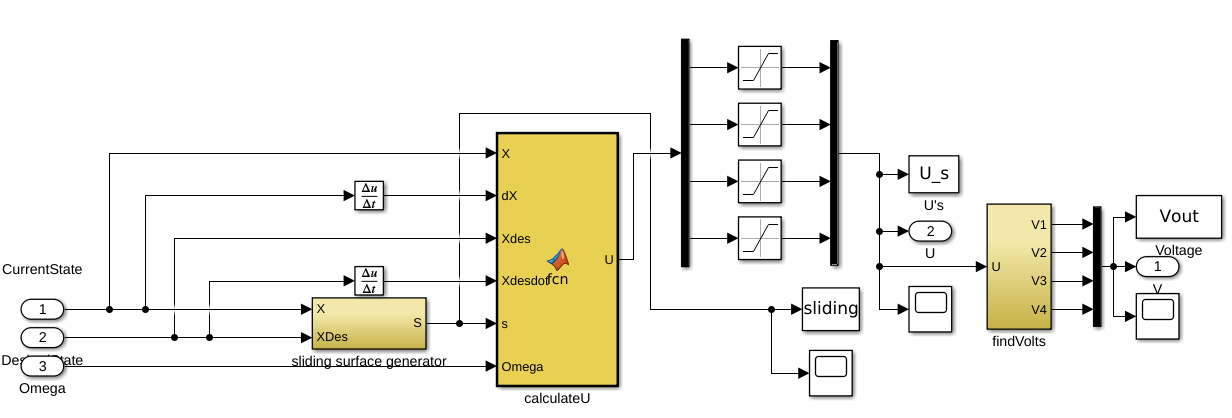
\includegraphics[width=0.70\textwidth]{controller.png}
\caption{\label{fig:controller}Block diagram of the controller}
\end{figure}
\end{center}

The \texttt{calculateU} block outputs the control inputs $U_i$ by implementing Equations \ref{eq:U}. Each $U$ is then fed into a saturation function which imposes constraints on the system to behave physically. More specifically, $U_1$ is bounded to greater than or equal to zero and less than an upper limit, as it is assumed that the rotors cannot output negative thrust and also have a maximum speed. If $U_1$ were negative, it would physically mean that the rotors start spinning in reverse, which is unrealistic. The other $U$ values have their magnitudes bounded at reasonable lmimits to ensure that the simulated system cannot impart unrealistic moments.

The resulting control inputs are then outputted from the controller subsystem, and are also fed into the \texttt{findVolts} block. This block outputs the rotor voltages as calculated with Equation \ref{eq:V2W}. These voltage values are also outputted from the controller subsystem.

\subsubsection{Dynamics Block Diagram}
The voltages and control inputs calculated in the controller subsystem are fed into the dynamics subsystem, which is shown in Figure \ref{fig:dynamics}. The \texttt{Motor Dynamics} subsystem implements first order dynamics for the motors to output $\Omega$. The motor 1 dynamics are shown in Figure \ref{fig:motor_dynamics}. While the majority of the dynamics subsystem was provided on Blackboard, the original blocks that calculated $U$ were removed as the control inputs were fed into the dynamics by the controller.

\begin{center}
\begin{figure}[H]
\captionsetup{width=1\textwidth}
\centering
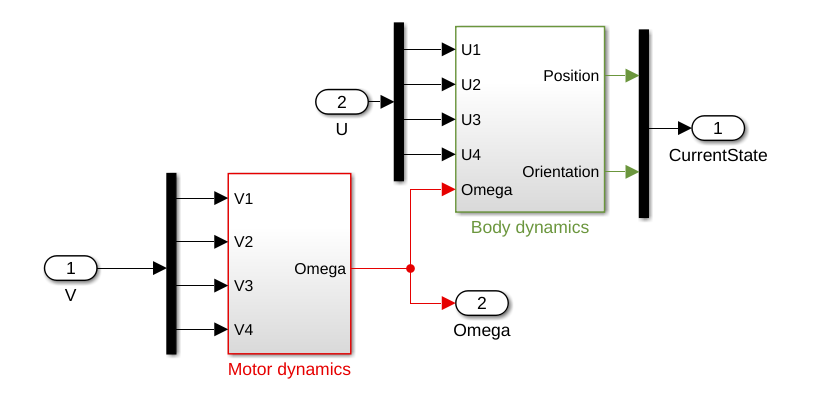
\includegraphics[width=0.70\textwidth]{dynamics.png}
\caption{\label{fig:dynamics}Block diagram of the dynamics}
\end{figure}
\end{center}


\begin{center}
\begin{figure}[H]
\captionsetup{width=1\textwidth}
\centering
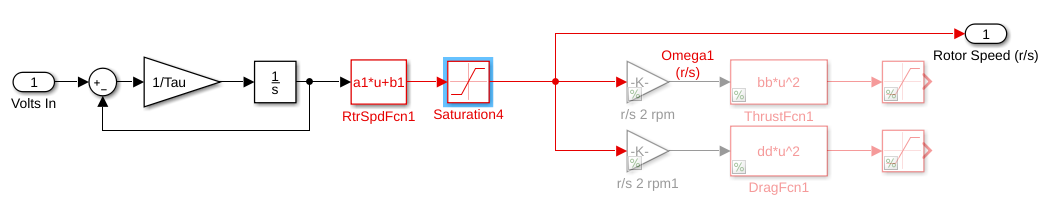
\includegraphics[width=0.70\textwidth]{motor_dynamics.png}
\caption{\label{fig:motor_dynamics}Block diagram of the motor dynamics}
\end{figure}
\end{center}

Once $\Omega$ is calculated in \texttt{Motor Dynamics}, the equations of motion as shown in Equations \ref{eq:inertialEOM} are simulated, with $\Omega$ and the $U_i$ values as inputs to the \texttt{Body Dynamics} block.

\subsubsection{Singularity Rejection} \label{sec:singularity_rejection}
As a result of the attitude of the quadrotor being represented with Euler angles, the controller suffers from issues with singularities. As can be seen in the $U_1$ equation in \ref{eq:U}, the entire equation for the thrust control input is divided by $\cos\phi\cos\theta$. Thus, when either $\phi$ or $\theta$ approach $\frac{\pi}{2}$, the $U_1$ control input approaches infinity. 

The occurrence of  singularities is avoided in the \texttt{Correct for Singularities} subsystem, the contents of which are shown in Figure \ref{fig:singularity_rejection}. The \texttt{Singularity in phi} and \texttt{Singularity in theta} blocks each take in the current (uncorrected) state and the desired state and they each output the state with a corrected angular term. If the $\phi$ or $\theta$ states are within an angular tolerance $t$ of $\frac{\pi}{2}$, then the subsystem outputs the state with the angle in question $2t$ closer to the desired state. The corrected $\phi$ and $\theta$ angles are overlaid on the raw angles in Figure \ref{fig:singularity_rejection_plots}. It should be noted that this process only affects the state that is input into the controller subsystem; the data from the output of the dynamics is not altered.

\begin{center}
\begin{figure}[H]
\captionsetup{width=1\textwidth}
\centering
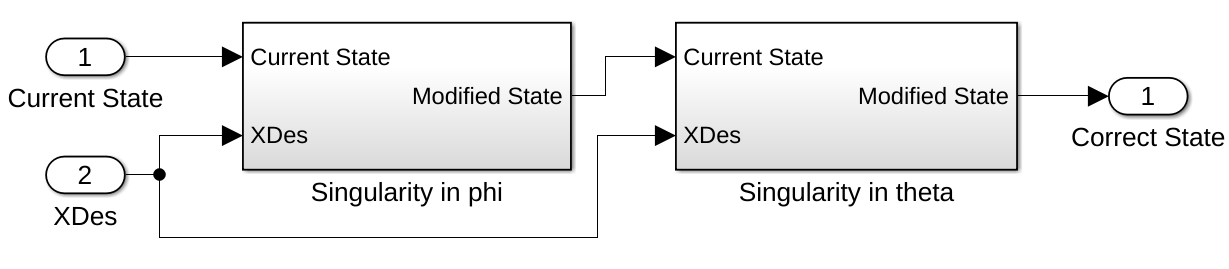
\includegraphics[width=0.70\textwidth]{singularity_rejection2.png}
\caption{\label{fig:singularity_rejection}Block diagram of the singularity rejection subsystem.}
\end{figure}
\end{center}

\begin{center}
\begin{figure}[H]
\captionsetup{width=1\textwidth}
\centering
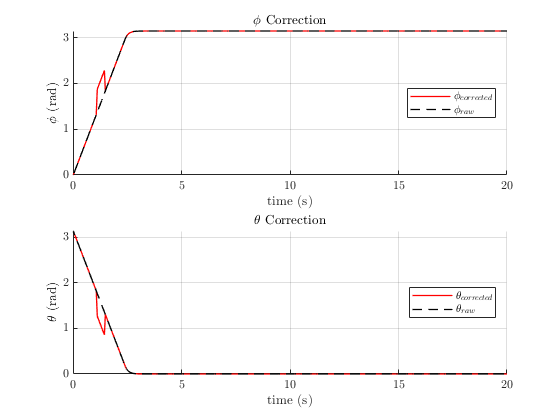
\includegraphics[width=0.70\textwidth]{singularity_rejection_plots.png}
\caption{\label{fig:singularity_rejection_plots}Plot of the corrected vs. raw $\phi$ and $\theta$ values}
\end{figure}
\end{center}


\subsection{Tuning Parameters} \label{sec:tuning}
In order to achieve the goal of stabilizing the quadcopter from random initial conditions, the tuning parameters of the controller had to be adjusted. The first test case that was used to tune the parameters was the "upside down throw into the air." The desired final state was $z_d = 12$, with all the other states equal to zero, and the initial conditions were as follows:

\begin{equation}
\bm x_0 = \begin{bmatrix}
0 & 0 & 0 & 0 & 2 & 5 & \pi & 0 & 0 & 0 & \frac{\pi}{2} & \pi
\end{bmatrix}^T
\end{equation}

The main two parameters that were varied were the proportional, integral, and derivative terms. The proportional term was increased to reduce the response time of the system, the integral term was increased to reduce steady state error, and the derivative term was increased to reduce overshoot. These parameters were tuned until a response with minimal ringing and steady state error was achieved. Table \ref{tab:tuning} demonstrates the results of this tuning.

\begin{table}[H]
\centering
\caption{Sliding Mode Control Tuning Parameters}
\label{tab:tuning}
\begin{tabular}{lllll}
         & $z$ & $\phi$ & $\theta$ & $\psi$ \\
$k_p$    & 50  & 50     & 50       & 50     \\
$k_i$    & 200 & 100    & 100      & 50     \\
$k_d$    & 10  & 10     & 10       & 10     \\
$\eta$   & 20  & 20     & 20       & 20     \\
$\kappa$ & 5   & 5      & 5        & 5     
\end{tabular}
\end{table}

\section{Results}
\subsection{Upside-Down Toss}
For the initial and desired conditions that were described in Section \ref{sec:tuning}, the results are shown in Figure \ref{fig:upside_down_throw}. As can be seen from the figure, the parameters chosen did not perfectly eliminate steady state error or overshoot. However, the rise time for all of the angles is well below one second, and steady state in the angles is reached by 2.5 seconds. The upwards step of 10 meters had a rise time of less than 2 seconds, and the system settles to the steady state height in under 5 seconds.

The results of this simulation show that the goal of this project was indeed met. The integral sliding mode controller was able to stabilize the quadrotor under the extreme initial condition of starting upside down. 

\begin{center}
\begin{figure}[H]
\captionsetup{width=1\textwidth}
\centering
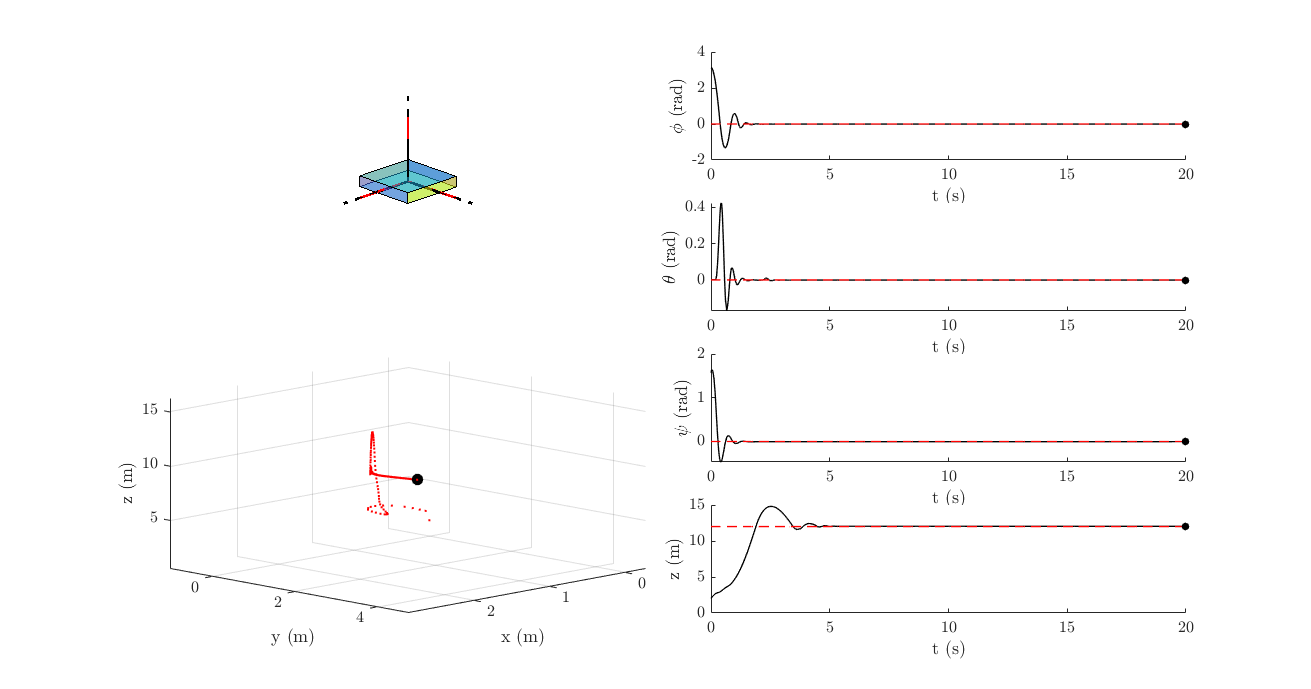
\includegraphics[width=1\textwidth]{upside_down_throw.png}
\caption{\label{fig:upside_down_throw}Results of the upside down throw}
\end{figure}
\end{center}

\subsection{Extreme Angular Rates}
To test the robustness of the controller, an incredibly large initial condition was used. The initial conditions and desired conditions for this result are the same as for the upside-down toss, except an initial pitch rate of 100 rad/s was used.

As can be seen, the controller does manage to bring the roll, pitch, yaw, and height states to constant values. However, there was significant steady state error. To combat this, all of the integral gains were doubled from the values stated in Section \ref{sec:tuning}, and the results of this test can be seen in Figure \ref{fig:crazyPitchRate}. Despite the incredibly high initial pitch rate, the controller does manage to bring the quadrotor to a steady angular state within 6 seconds, and a steady height in under 12 seconds. 

It is interesting to note that despite the quadrotor's nonzero steady state angles, it was able to bring itself to a steady-state height. This makes sense, since height is one of the controlled variables. However, one of the major shortcomings of this controller is immediately obvious. Since x and y position are not controlled, any steady state error in the angular states causes the quadcopter to fly at a steady rate in the horizontal plane. Thus, in applications where the horizontal position of the quadrotor is important, attitude control of the quadrotor is not necessarily the ideal method of stabilization. 

\begin{center}
\begin{figure}[H]
\captionsetup{width=1\textwidth}
\centering
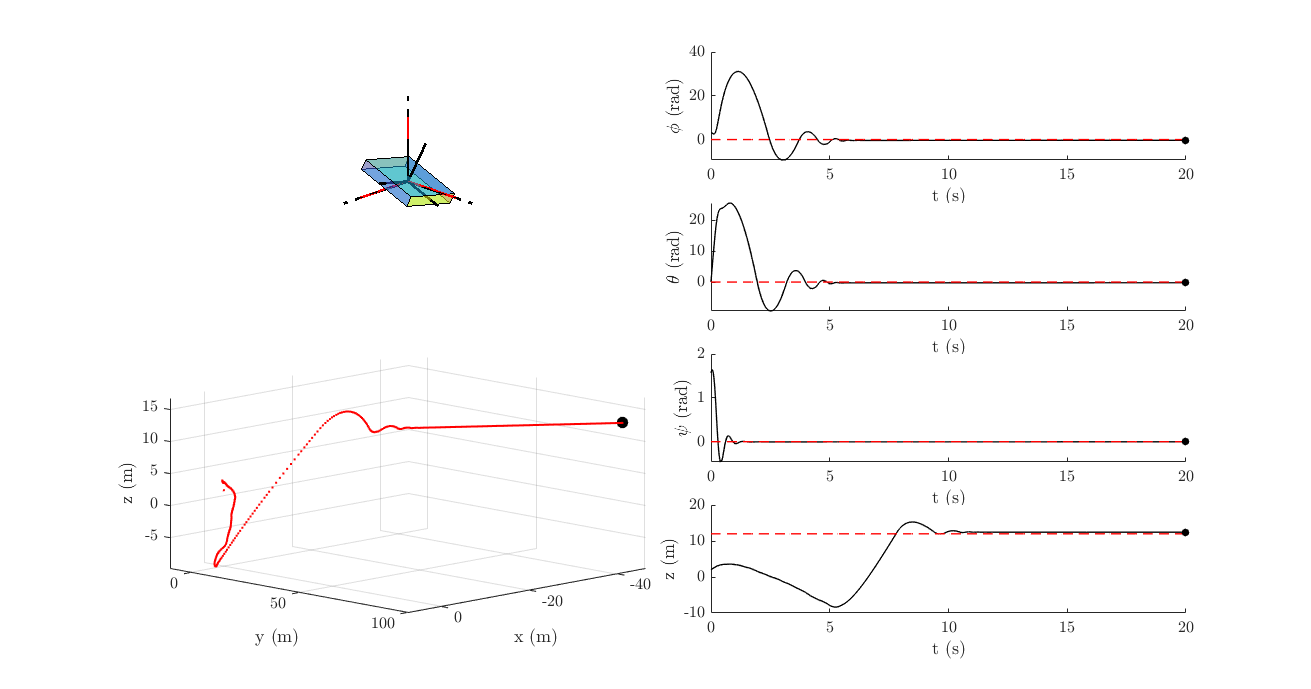
\includegraphics[width=1\textwidth]{crazyPitchRate.png}
\caption{\label{fig:crazyPitchRate}Results of the extreme angular rates test}
\end{figure}
\end{center}

\subsection{2D Weaving}
While explicit position control in the horizontal plane is not possible with the implemented integral sliding mode control, if a trajectory in the horizontal plane could be calculated based on the variation of the angular parameters, then position control in the horizontal plane could be attempted implicitly. This test case was to test the ability of the controller to follow a predetermined attitude time history, while also attempting to have the quadcopter follow a pseudo-sinusoidal path in the horizontal plane. The initial conditions of this test are all zeros, the integral gains remain at the same values as in the extreme pitch rate test, and the desired state was as follows, where $a=1$ and $b=1$ are constants with units of radians.

\begin{equation}
\bm x_0 = \begin{bmatrix}
0 & 0 & 0 & 0 & 0 & 0 & a\cos t & 0 & -\frac{\pi}{6}& 0 & b\sin t & 0
\end{bmatrix}^T
\end{equation}

As can be seen by Figure \ref{fig:weaving}, the integral sliding mode controller is able to accurately follow the desired roll and yaw angles. However, there is interesting behavior in the pitch angle. The pitch angle does not remain steadily at $-\pi/6$ as would be expected. Instead, the angle seems to be perturbed around 8 and 9 seconds into the simulation, as well as around 14 and 15 seconds. 

This could be due to chattering of the sliding mode controller. While the $\tanh$ terms in the control inputs were used to mitigate chattering while the system was moving along the sliding surface, the possibility of chattering still exists. One way to potentially eliminate the chattering during this test case could be to introduce an additional term inside the $\tanh$ function within the control inputs, which could scale the argument of the function such that chattering is eliminated.

\begin{center}
\begin{figure}[H]
\captionsetup{width=1\textwidth}
\centering
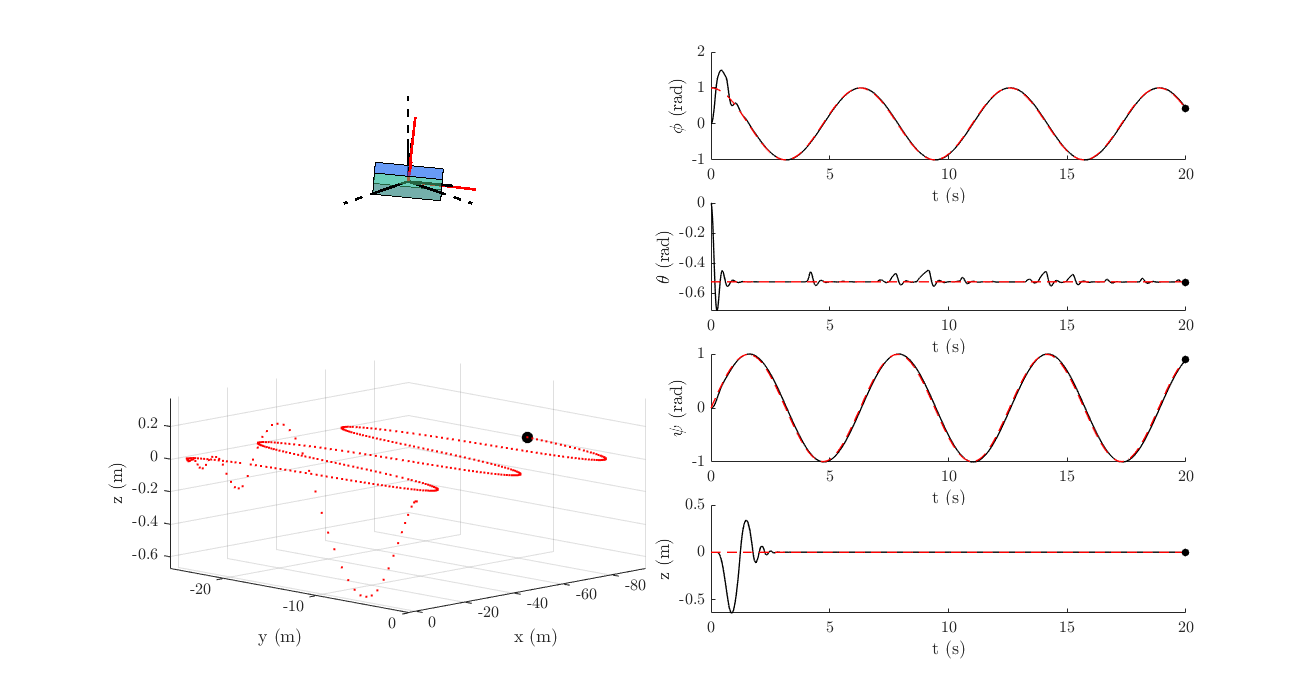
\includegraphics[width=1\textwidth]{weaving.png}
\caption{\label{fig:weaving}Results of the weaving test}
\end{figure}
\end{center}

\subsection{Step Disturbance Rejection}
It was desired to test the disturbance rejection abilities of the implemented controller. Thus, the weaving case was attempted with a wind disturbance in the $z$ direction. Wind was modeled as follows:
\begin{equation}
F_{z-wind} = -k(v_{z-wind} - v_{z-current})
\end{equation}
and the disturbance in the z velocity was added into the body dynamics block as can be seen in Figure \ref{fig:wind_block}. In this test case, a wind velocity of 40 m/s in the z direction is applied from 4 to 5 seconds. 

\begin{center}
\begin{figure}[H]
\captionsetup{width=1\textwidth}
\centering
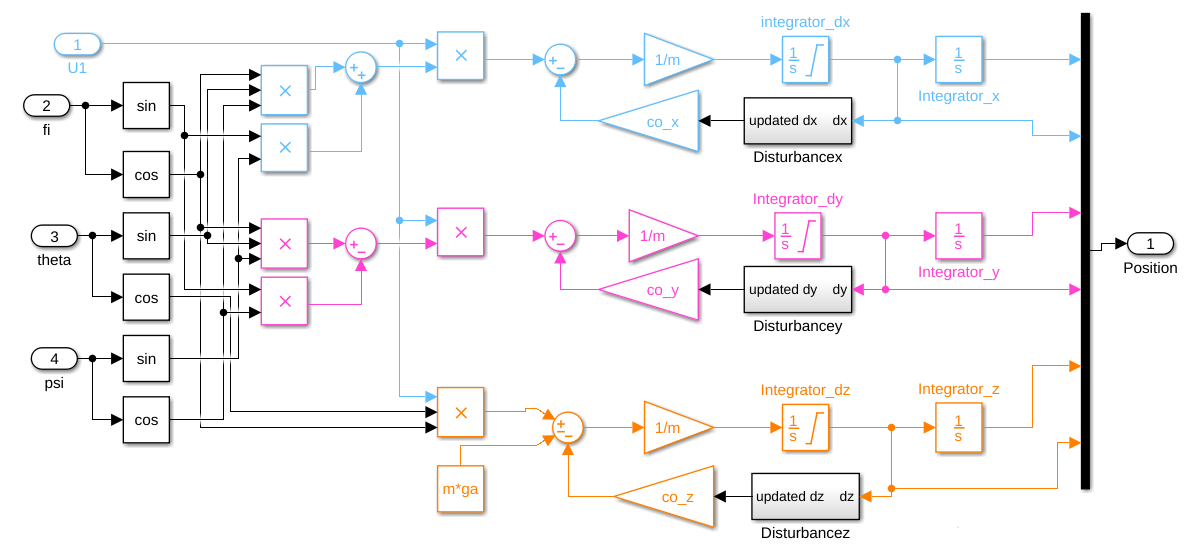
\includegraphics[width=1\textwidth]{disturbance_simulink.png}
\caption{\label{fig:wind_block}Modeling of wind disturbance in Simulink}
\end{figure}
\end{center}

The desired states were the same as in the 2D weaving case, and the initial conditions that were applied for this test case were:

\begin{equation}
\bm x_0 = \begin{bmatrix}
0 & 0 & 0 & 0 & 10 & 0 & 1 & 0 & -\frac{\pi}{6}& 0 & 0 & 1
\end{bmatrix}^T
\end{equation}

As can be seen in Figure \ref{fig:zdisturbance}, the disturbance causes an increase in the quadcopter's height of almost 26 meters, and the controller brings the drone back to steady state in under 10 seconds. However, the result of the disturbance is that the steady state error at the end of the simulation is -0.4 meters. It is clear from this result, as well as the previous ones, that the gains of the controller need to be better optimized to reduce steady state errors. 

The chattering phenomenon is also more evident in the step disturbance test. The values of $\theta$ vary up to 0.1 rad, which is a significant amount of chatter. As mentioned in the 2D weaving section, this could be corrected by adding an additional tuning parameter in the $\tanh$ function that could be adjusted to smooth out the jagged behavior.

\begin{center}
\begin{figure}[H]
\captionsetup{width=1\textwidth}
\centering
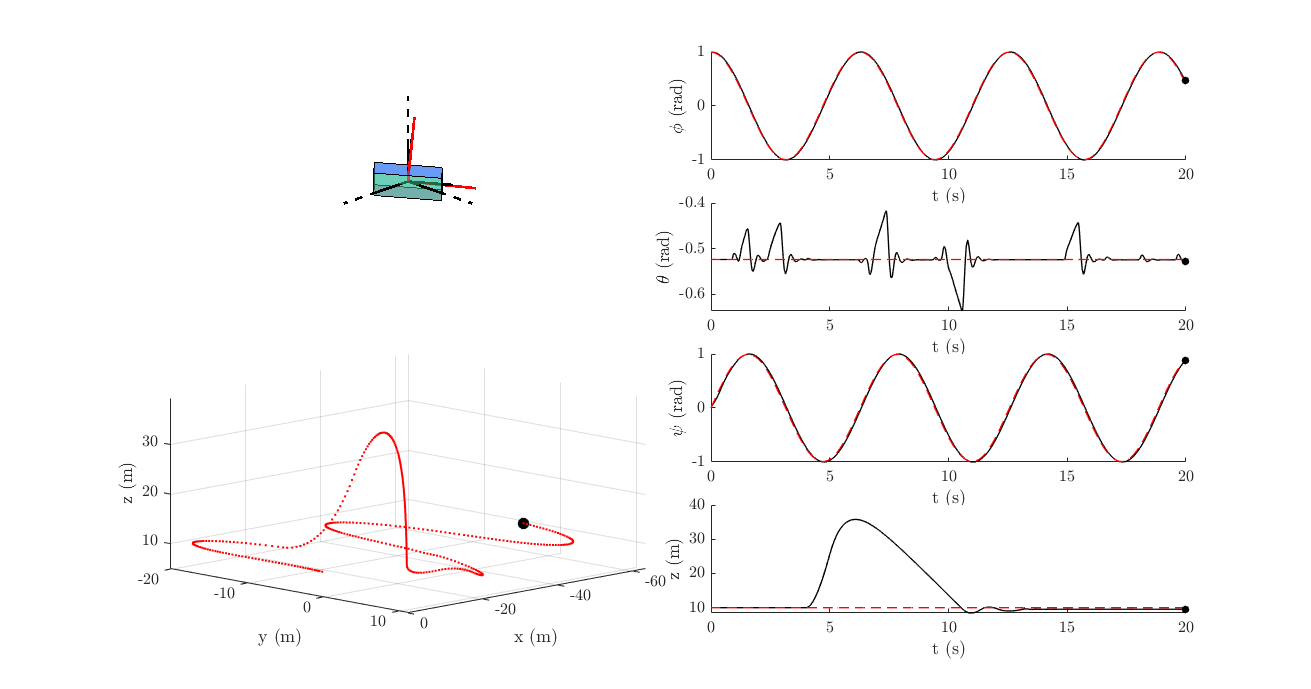
\includegraphics[width=1\textwidth]{zdisturbance.png}
\caption{\label{fig:zdisturbance}Results of modeling a disturbance in the z direction.}
\end{figure}
\end{center}


\section{Conclusion}
Through the work documented in this paper, an integral sliding mode controller has been designed to stabilize the attitude and height of a quadrotor helicopter under arbitrary initial conditions. The controller converged to steady state values quickly, rejected disturbances (albeit with some steady state error), and was effective even under very difficult initial conditions, such as being thrown while the drone was upside down. However, it was determined that pure attitude control coupled with height control of a quadrotor is not the ideal method of stabilization, as significant movement can occur in the uncontrolled horizontal plane due to even slight nonzero steady state errors in the roll, pitch, and yaw angles. Improvements can be made to the controller by seeking analytical ways of optimizing the values of the tuning parameters to improve the steady state error. Additionally, another major improvement would come from expressing positional rates in terms of the other states in order to also control and stabilize the horizontal position of the quadrotor.

\newpage
\begin{thebibliography}{9}
\bibitem{SudhirSwarup}
Sudhir and A. Swamp, “Second order sliding mode control for quadrotor,” \textit{2016 IEEE First International Conference on Control, Measurement and Instrumentation (CMI)}, 2016.

\bibitem{twisty}
H. Jayakrishnan, “Position and Attitude control of a Quadrotor UAV using Super Twisting Sliding Mode,” \textit{IFAC-PapersOnLine}, vol. 49, no. 1, pp. 284–289, 2016.

\bibitem{SMCControlObservation} 
Y. Shtessel, C. Edwards, L. Fridman, and A. Levant, \textit{Sliding Mode Control and Observation}. New York, NY: Springer, Imprint: Birkh$\ddot{a}$user, 2014.

\bibitem{camacho}
O. Camacho, R. Rojas, and W. García-Gabín, “Some long time delay sliding mode control approaches,” \textit{ISA Transactions}, vol. 46, no. 1, pp. 95–101, 2007.

\bibitem{khalil}
Khalil, H. (2002). \textit{Nonlinear systems}. Upper Saddle River, NJ: Prentice Hall.
\end{thebibliography}



\newpage
\appendix
\section{runMain.m}
\lstinputlisting[style=Matlab-editor]{runMain.m}

\section{QuadrotorConstants.m}
\lstinputlisting[style=Matlab-editor]{QuadrotorConstants.m}

\section{TuningParameters.m}
\lstinputlisting[style=Matlab-editor]{TuningParameters.m}

\section{animateQuadrotor.m}
\lstinputlisting[style=Matlab-editor]{animateQuadrotor.m}

\end{document}









